% =============================================================================
% A Microcoded Command Processor for a Flexible FPGA Butterfly Engine
%
% Build:  pdflatex paper.tex  (twice)
% All numbers, tables and timeline bars are generated from the simulator by
% gen_paper_data.py into generated/*.tex -- nothing quantitative is hand-typed.
% Author list is a placeholder: edit before circulating.
% =============================================================================
\documentclass[twocolumn,10pt]{article}

\usepackage[letterpaper,margin=0.72in,columnsep=0.26in]{geometry}
\usepackage{mathptmx}
\usepackage[scaled=0.92]{helvet}
\usepackage{courier}
\usepackage{amsmath,amssymb}
\usepackage{booktabs,multirow,array}
\usepackage{xcolor}
\usepackage{tikz}
\usepackage{pgfplots}
\pgfplotsset{compat=1.17}
\usetikzlibrary{positioning,arrows.meta,calc,fit,decorations.pathreplacing,matrix}
\usepackage{bytefield}
\usepackage{listings}
\usepackage[font=small,labelfont=bf,skip=4pt]{caption}
\usepackage{microtype}
\usepackage[hidelinks]{hyperref}
\usepackage{titlesec}
\titlespacing*{\section}{0pt}{8pt plus 2pt}{4pt}
\titlespacing*{\subsection}{0pt}{6pt plus 2pt}{3pt}

\newcommand{\HeadlineCycles}{15,360}
\newcommand{\HeadlineUs}{51.2}
\newcommand{\CfgCycles}{64,320}
\newcommand{\CfgMs}{0.214}
\newcommand{\CfgUs}{214.4}
\newcommand{\CfgSps}{4,664}
\newcommand{\PrsMux}{256}
\newcommand{\PrsRegs}{2,560}
\newcommand{\PrsMuxBig}{1,408}
\newcommand{\XbarMuxBig}{16,256}
\newcommand{\SqnrDb}{48.4}
\newcommand{\WeCycles}{16}
\newcommand{\WeBrev}{4}
\newcommand{\WeStages}{4}
\newcommand{\WeCPS}{4}
\newcommand{\ProgCmds}{104}
\newcommand{\ProgBytes}{3,328}
\newcommand{\ProgDmaIn}{1}
\newcommand{\ProgDmaOut}{1}
\newcommand{\ProgCompute}{102}
\newcommand{\PynqUs}{878}
\newcommand{\PynqOvh}{281}
\newcommand{\PynqSps}{1,139}
\newcommand{\StaticUs}{252.5}
\newcommand{\StaticOvh}{9.6}
\newcommand{\TunedUs}{250.3}
\newcommand{\TunedOvh}{8.7}
\newcommand{\MmioOvh}{12.0}
\newcommand{\PeakSps}{4,664}
\newcommand{\TunedBatchTenSps}{4,303}
\newcommand{\TunedBatchTenPct}{92}
\newcommand{\StaticBatchTenSps}{3,981}
\newcommand{\SeqLut}{3,640}
\newcommand{\SeqBram}{2}
\newcommand{\SeqPct}{2.4}
\newcommand{\TotLut}{156,193}
\newcommand{\LinkNeed}{0.62}
\newcommand{\LinkHave}{6.4}
\newcommand{\LinkPct}{10}
\newcommand{\InKB}{128}
\newcommand{\OutKB}{2.0}
\newcommand{\TimelineEnd}{480.7}
\newcommand{\TimelineTwoPerInf}{240.4}
\newcommand{\GlueUs}{16.0}
\newcommand{\GluePct}{7}

\newcommand{\batchpeak}{(1,4664) (2,4664) (4,4664) (6,4664) (8,4664) (10,4664)}
\newcommand{\batchpynq}{(1,1139) (2,1169) (4,1185) (6,1191) (8,1194) (10,1195)}
\newcommand{\batchstatic}{(1,3961) (2,3972) (4,3978) (6,3980) (8,3981) (10,3981)}
\newcommand{\batchtuned}{(1,3995) (2,4160) (4,4248) (6,4279) (8,4294) (10,4303)}
\newcommand{\prefetchsweep}{(1,254.5) (2,254.5) (4,251.3) (8,250.3) (16,250.3) (32,250.3)}
\newcommand{\prscost}{(4,14) (8,40) (16,104) (32,256) (64,608) (128,1408)}
\newcommand{\xbarcost}{(4,12) (8,56) (16,240) (32,992) (64,4032) (128,16256)}

\newcommand{\tracetablerows}{%
0 & 3 & 0 & (0,8,2,10) & (0,1,2,3) & (0,2,0,2) & 0 & 0 & (0,2) \\
0 & 3 & 1 & (1,9,3,11) & (1,2,3,0) & (2,0,2,0) & 1 & 0 & (1,3) \\
0 & 3 & 2 & (4,12,6,14) & (1,2,3,0) & (3,1,3,1) & 1 & 0 & (4,6) \\
0 & 3 & 3 & (5,13,7,15) & (2,3,0,1) & (1,3,1,3) & 2 & 0 & (5,7) \\
\addlinespace[1pt]
1 & 2 & 0 & (0,4,2,6) & (0,1,2,3) & (0,1,0,1) & 0 & 0 & (0,2) \\
1 & 2 & 1 & (1,5,3,7) & (1,2,3,0) & (1,0,1,0) & 1 & 0 & (1,3) \\
1 & 2 & 2 & (8,12,10,14) & (1,2,3,0) & (3,2,3,2) & 1 & 0 & (4,6) \\
1 & 2 & 3 & (9,13,11,15) & (2,3,0,1) & (2,3,2,3) & 2 & 0 & (5,7) \\
\addlinespace[1pt]
2 & 1 & 0 & (0,2,1,3) & (0,2,1,3) & (0,0,0,0) & 0 & 1 & (0,1) \\
2 & 1 & 1 & (4,6,5,7) & (1,3,2,0) & (1,1,1,1) & 1 & 1 & (2,3) \\
2 & 1 & 2 & (8,10,9,11) & (1,3,2,0) & (2,2,2,2) & 1 & 1 & (4,5) \\
2 & 1 & 3 & (12,14,13,15) & (2,0,3,1) & (3,3,3,3) & 2 & 1 & (6,7) \\
\addlinespace[1pt]
3 & 0 & 0 & (0,1,2,3) & (0,1,2,3) & (0,0,0,0) & 0 & 0 & (0,1) \\
3 & 0 & 1 & (4,5,6,7) & (1,2,3,0) & (1,1,1,1) & 1 & 0 & (2,3) \\
3 & 0 & 2 & (8,9,10,11) & (1,2,3,0) & (2,2,2,2) & 1 & 0 & (4,5) \\
3 & 0 & 3 & (12,13,14,15) & (2,3,0,1) & (3,3,3,3) & 2 & 0 & (6,7) \\}

\newcommand{\programheadrows}{%
0 & \texttt{bs.load} & IQ chunk 0 & dma\_in & 128\,KB & -- \\
1 & \texttt{bs.pow} & S2 & compute & 256\,cyc & 0 \\
2 & \texttt{bs.pow} & S4 & compute & 256\,cyc & 0 \\
3 & \texttt{bs.pow} & S6 & compute & 256\,cyc & 0 \\
4 & \texttt{bs.pow} & S8 & compute & 256\,cyc & 0 \\
5 & \texttt{bs.bfly} & 4 x 32768-point FFT & compute & 15,360\,cyc & 1,2,3,4 \\
6 & \texttt{bs.brev} & write-back pass & compute & 1,024\,cyc & 5 \\
7 & \texttt{bs.mag} & branch 0 & compute & 256\,cyc & 6 \\
8 & \texttt{bs.bfly} & expansion 0 & compute & 3,072\,cyc & 7 \\
\multicolumn{6}{c}{$\vdots$ (8 branches $\times$ 11 descriptors)} \\
103 & \texttt{bs.store} & features & dma\_out & 2\,KB & 18..102 \\
}

\newcommand{\programhexrows}{%
\texttt{bs.load} & \shortstack[l]{\texttt{00000001 001f0000 00000000 00000000}\\\texttt{00000000 00008000 00000000 00000000}} & load one 32{,}768-sample IQ record to BSPM word 0 \\[2.5pt]
\texttt{bs.bfly (FFT)} & \shortstack[l]{\texttt{0f000010 000e0000 00000000 00000000}\\\texttt{00000000 00000000 00000004 00000005}} & four 32{,}768-point FFTs, twiddles at CRAM 0 \\[2.5pt]
\texttt{bs.store (BITREV)} & \shortstack[l]{\texttt{00000103 001f0000 00000000 00000000}\\\texttt{00000000 00008000 00000000 00000006}} & bit-reversal write-back fused into the store \\[2.5pt]
\texttt{bs.bfly (BL)} & \shortstack[l]{\texttt{05020810 00040000 00000000 00000000}\\\texttt{00000040 00000000 00000400 00000009}} & 1{,}024 length-32 BL transforms, fused ReLU \\[2.5pt]
\texttt{bs.bfly (short)} & \shortstack[l]{\texttt{03030010 00020002 00000000 00000000}\\\texttt{00000080 00000000 00001000 00000008}} & 4{,}096 length-8 transforms, $P_{sub}{=}4$ folded per pass \\[2.5pt]
}

\newcommand{\breakdownrows}{%
CC extraction: 4 $\times$ 32768-point FFT & 15,360 & 51.20 \\
bit-reversal write-back & 1,024 & 3.41 \\
8 $\times$ feature expansion (len 8, $\times$4) & 24,576 & 81.92 \\
8 $\times$ MLP-0-\{0,1\} (len 32, 1024 rows) & 20,480 & 68.27 \\
8 $\times$ MLP-1-\{0,1\} (len 32, 128 rows) & 2,560 & 8.53 \\
8 $\times$ MLP-2-\{0,1\} (len 32, 16 rows) & 320 & 1.07 \\
\midrule
total & 64,320 & 214.4 \\}

\newcommand{\platformrows}{%
PYNQ / Jupyter flow & 878.3 & 281.2 & 1,139 & host \\
MMIO per descriptor (Linux) & 258.1 & 12.0 & 3,874 & compute \\
ring rebuilt per inference & 252.5 & 9.6 & 3,960 & compute \\
static ring + doorbell & 252.5 & 9.6 & 3,961 & compute \\
static ring, split queues, streamed input & 250.3 & 8.7 & 3,995 & compute \\
}


\definecolor{barA}{RGB}{70,110,180}
\definecolor{barB}{RGB}{220,140,60}
\definecolor{blkmem}{RGB}{225,238,250}
\definecolor{blkcomp}{RGB}{252,235,215}
\definecolor{blkctl}{RGB}{228,246,228}
\definecolor{blkio}{RGB}{240,240,240}

\lstset{basicstyle=\ttfamily\scriptsize,columns=fullflexible,
        keepspaces=true,frame=single,framesep=3pt,xleftmargin=3pt,
        commentstyle=\color{black!55}\itshape,language={}}

\newcommand{\bsm}{\mathrm{bsm}}
\newcommand{\ins}{\mathrm{ins}}
\newcommand{\Pbu}{P_{bu}}
\newcommand{\Pbe}{P_{be}}
\newcommand{\Psub}{P_{sub}}
\newcommand{\PN}{P_{N}}
\newcommand{\op}[1]{\texttt{#1}}

\title{\LARGE\bfseries A Microcoded Command Processor for a Flexible
FPGA Butterfly Engine}
\author{%
Draft manuscript --- author list to be completed\\
\normalsize Computer Engineering Laboratory, The University of Sydney}
\date{}

\begin{document}
\maketitle

% ---------------------------------------------------------------------------
\begin{abstract}
\noindent
FlexBE is a fixed-function FPGA accelerator that executes both long fast
Fourier transforms and butterfly-linear neural-network layers on a single
radix-2 datapath, with the layer sequence fixed at synthesis.  An architecture
is described that makes the accelerator software programmable while leaving the
datapath untouched: a microcoded command processor, implemented as a small
sequencer in the programmable logic, executes a queue of 32-byte descriptors
that cover data movement, butterfly transforms, and the pointwise operations of
the target workload.  Two properties of the design are emphasised.  The unit of
issue is the layer rather than the individual operation, which is appropriate
because the datapath retires 64 butterflies per cycle; a single \op{bs.bfly}
descriptor accordingly retires the engine's entire closed-form cycle count.
Descriptors name memories and transforms but not bank indices, switch settings,
or cycle schedules, so the conflict-free addressing scheme may be revised
without invalidating existing programs.  The datapath, the architectural state,
the descriptor format, and its decode are presented, and a 16-point transform
is traced through the machine cycle by cycle.  On a model of a Zynq
UltraScale+ ZCU104, the sequencer requires \SeqLut{} LUTs
(\SeqPct\% above the fixed-function system) and completes a
\ProgCmds-descriptor automatic-modulation-classification inference within
\TunedOvh\% of the hardwired datapath, sustaining \TunedBatchTenPct\% of peak
throughput at a batch size of ten.  The same model indicates that the
interactive Python flow used to benchmark the original accelerator is limited by
processing-system software rather than by the accelerator, and overstates
single-batch latency by a factor of $3.5$.
\end{abstract}

% ---------------------------------------------------------------------------
\section{Introduction}\label{sec:intro}

Edge radio-frequency machine learning (RFML) combines two stages with very
different computational profiles.  The first is a small number of long
transforms; cyclostationary feature extraction, for example, requires four
32{,}768-point FFTs per classification.  The second is a large number of short,
highly parallel linear layers.  FlexBE~\cite{flexbe} accommodates both on one
datapath by exploiting the butterfly factorisation of Dao et
al.~\cite{dao2019butterfly}, in which an FFT stage and a trained
butterfly-linear (BL) layer are the same dataflow evaluated with different
$2{\times}2$ coefficients.  On an AMD ZCU104, the resulting system computes four
32{,}768-point FFTs in \HeadlineCycles{} cycles (\HeadlineUs\,$\mu$s at
300\,MHz) and a complete BSPNet inference in \CfgMs\,ms.

The published system is fixed function.  The sequence of layers, together with
their lengths and their interleaving, is embedded in a hardwired top-level state
machine, so that any change to the model requires re-synthesis.  The question
addressed here is what minimal architecture converts the layer graph into
runtime data.  The answer taken is a microcoded command processor: a
descriptor-driven sequencer placed in the programmable logic, following the
tradition of microprogrammed control~\cite{wilkes1953} and of the command
processors found in contemporary
accelerators~\cite{nvdla,gemmini,vta,tpu}.

Because the datapath retires 64 butterflies per cycle, fine-grained instructions
cannot supply work fast enough to be profitable, and on a Zynq MPSoC the hard
Cortex-A53 cluster in any case provides no custom-instruction port; both points
are quantified in \S\ref{sec:granularity}.  The remaining design choice is the
position of the command boundary, and it is argued here that the boundary
belongs at the layer.  Three consequences of this choice organise the design.
First, a single \op{bs.bfly} descriptor carries the transform length $l$, the
sub-parallelism $\Psub$, and the batch $\PN$, and retires the engine's
closed-form cycle count (Eq.~\ref{eq:cycles}); the accelerator's
runtime-reconfigurable parameters thus become operand fields rather than
configuration registers.  Second, no opcode names a RAM bank, a switch setting,
or a cycle index, so that the conflict-free addressing of \S\ref{sec:engine} is
derived at decode time and remains free to change beneath the instruction set.
Third, the pointwise operations are made architectural: magnitude computation
alone accounts for 26\% of the published system's LUTs, and in the absence of
\op{bs.pow}, \op{bs.mag}, and \op{bs.pool} descriptors every feature would be
returned to memory and re-read, forfeiting the advantage of the fused datapath.

The contributions of the paper are as follows.  The architecture of the command
processor is described, including its datapath, architectural state,
per-resource descriptor queues, and completion path (\S\ref{sec:arch}).  The
microcode format is specified as a 32-byte descriptor, with its field semantics,
encodings, and decode into engine control (\S\ref{sec:format}).  A worked
example is given at two scales: a 16-point transform traced cycle by cycle
through banks, switches, and butterfly units, and a complete
\ProgCmds-descriptor inference with its execution timeline (\S\ref{sec:worked}).
Finally, an evaluation is carried out on a validated cycle-level model, from
which it emerges that the throughput shortfall observed in the published system
is attributable chiefly to processing-system software rather than to the
accelerator (\S\ref{sec:eval}).

% ---------------------------------------------------------------------------
\section{Background: the Butterfly Engine}\label{sec:engine}

The engine driven by the command processor is summarised in this section, in
the form implemented by the simulator.  Each property stated below is checked by
the accompanying test suite.

\subsection{Shift-down banked memory}\label{sec:mem}

In-flight data is held in $P = 2\Pbu$ single-port RAM banks.  Element index $I$
of an $N = 2^n$-point working set is stored at depth $a_x$ of bank $a_y$,
\begin{equation}
a_x = I \gg m,\qquad
a_y = \bsm(I) = \big[\mathrm{pc}(I \gg m) + (I \bmod 2^m)\big] \bmod 2^m,
\label{eq:bsm}
\end{equation}
where $m = \log_2 2\Pbu$ and $\mathrm{pc}$ denotes the population count.
Equation~\ref{eq:bsm} admits a geometric reading: a RAM row consists of $2^m$
consecutive indices, and row $H$ is stored cyclically rotated by $\mathrm{pc}(H)$
banks (Fig.~\ref{fig:memory}).  The conflict-freedom results that follow are
consequences of this observation.

\begin{figure}[t]
\centering
\resizebox{0.97\linewidth}{!}{%
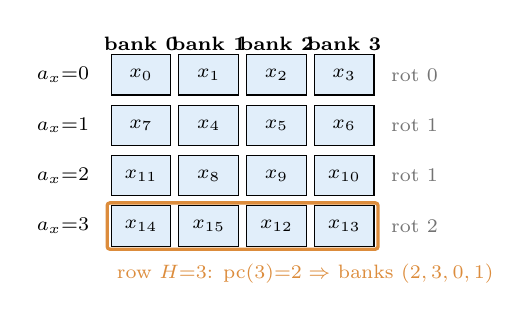
\begin{tikzpicture}[x=8.6mm,y=6.4mm,font=\scriptsize]
  \foreach \b in {0,...,3} {
    \node[font=\scriptsize\bfseries] at (\b,0.62) {bank \b};
  }
  % depth rows: element index placed at (bank, -depth)
  % depth0: 0,1,2,3 ; depth1: b0=7,b1=4,b2=5,b3=6
  % depth2: b0=11,b1=8,b2=9,b3=10 ; depth3: b0=14,b1=15,b2=12,b3=13
  \foreach \d/\ea/\eb/\ec/\ed/\rot in
    {0/0/1/2/3/0, 1/7/4/5/6/1, 2/11/8/9/10/1, 3/14/15/12/13/2} {
    \node[anchor=east] at (-0.62,-\d) {$a_x{=}\d$};
    \node[anchor=west,text=black!55] at (3.55,-\d) {rot $\rot$};
    \foreach \b/\e in {0/\ea,1/\eb,2/\ec,3/\ed} {
      \draw[fill=blkmem] (\b-0.44,-\d-0.4) rectangle (\b+0.44,-\d+0.4);
      \node at (\b,-\d) {$x_{\e}$};
    }
  }
  % highlight row H=3 (elements 12..15), rotation 2
  \draw[very thick,barB,rounded corners=1pt] (-0.5,-3.46) rectangle (3.5,-2.54);
  \node[barB,anchor=west,font=\scriptsize] at (-0.5,-3.95)
    {row $H{=}3$: $\mathrm{pc}(3){=}2 \Rightarrow$ banks $(2,3,0,1)$};
\end{tikzpicture}}
\caption{Shift-down storage (Eq.~\ref{eq:bsm}) for $N{=}16$, $\Pbu{=}2$
($P{=}4$ banks).  Row $H$ holds elements $4H..4H{+}3$ rotated by
$\mathrm{pc}(H)$ banks, so that any complete row, and, as shown in
\S\ref{sec:sched}, any scheduled cycle, touches every bank exactly once.}
\label{fig:memory}
\end{figure}

\subsection{The per-cycle schedule and the PRS}\label{sec:sched}

A decimation-in-frequency radix-2 dataflow is used.  Stage $k$ of an $n$-stage
transform pairs indices differing in the hole bit $h = n{-}1{-}k$, so that
natural-order input produces bit-reversed output; the write-back path of
\S\ref{sec:brev} restores the natural order.  In each cycle, $2\Pbu$ operands
are read, permuted into butterfly-slot order, transformed by $\Pbu$ radix-2
units, inverse-permuted, and written back in place (Fig.~\ref{fig:datapath}).

Under Eq.~\ref{eq:bsm}, conflict-free access requires two regimes, both of
which are produced by the closed-form control
$\mathsf{cycle\_control}(n,\Pbu,k,j)$.  Writing
$\ins(x,p) = ((x \gg p) \ll (p{+}1)) \,|\, (x \bmod 2^p)$ for the insertion of
a zero bit at position $p$, the control is
\begin{align*}
h < m:\;& H \leftarrow j; \quad
  I^i[2t] \leftarrow (H \ll m) + \ins(t,h); \quad S^i \leftarrow h\\
h \ge m:\;& e \leftarrow j \bmod 2;\;\; H \leftarrow \ins(j \gg 1,\, h{-}m);\\
 & I^i[2t] \leftarrow (H \ll m) + 2t + e; \quad S^i \leftarrow 0\\
\text{both}:\;& I^i[2t{+}1] \leftarrow I^i[2t] + 2^h;\quad
  R^i \leftarrow \bsm(I^i[0]).
\end{align*}
When $h<m$, a cycle reads one complete row, whose banks
$(\mathrm{pc}(H)+\mathit{low}) \bmod 2^m$ are pairwise distinct; slot $j$ then
reads bank $(\pi_h[j]+\mathrm{pc}(H)) \bmod 2^m$, which is a fixed stride
permutation composed with a rotation.  When $h\ge m$, the partner element lies
in row $H+2^{h-m}$, whose population count is greater by exactly one, so that
slot $j$ reads bank $(\mathrm{pc}(H)+e+j)\bmod 2^m$, a pure rotation.  The
required permutation therefore factors in every case as
$\mathbf{P}_f = \mathbf{P}_s \times \mathbf{P}_r$ with at most $m$ subset states,
and the switch reduces to a barrel shifter followed by a log-depth subset
network (Fig.~\ref{fig:prs}).  Its cost is $mP + (m{+}1)2^{m-1}$ two-input
multiplexers per bit, i.e.\ $\Theta(m\Pbu)$ and \PrsMux{} at $\Pbu{=}16$,
compared with the $\Theta(\Pbu^2)$ of a general crossbar over the same ports
(Fig.~\ref{fig:prscost}).  Each branch emits exactly $N/2\Pbu$ cycles per stage
and visits every index once.

\begin{figure}[t]
\centering
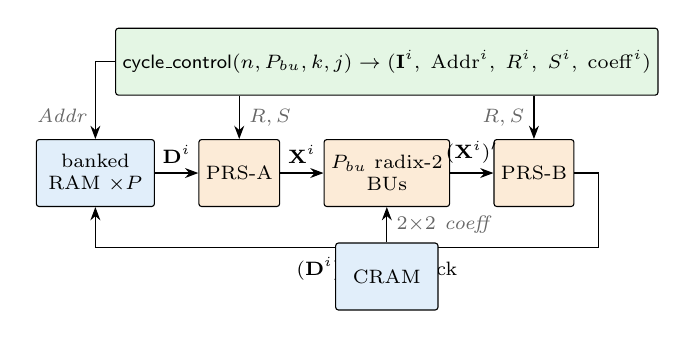
\begin{tikzpicture}[font=\scriptsize,>=Stealth,
  blk/.style={draw,rounded corners=1pt,minimum height=8.5mm,inner sep=2.5pt,align=center},
  lbl/.style={font=\scriptsize\itshape,text=black!60}]
  \node[blk,fill=blkmem,minimum width=15mm]   (ram)  {banked\\RAM $\times P$};
  \node[blk,fill=blkcomp,right=5.5mm of ram]  (prsa) {PRS-A};
  \node[blk,fill=blkcomp,right=5.5mm of prsa,minimum width=13mm] (bu)
        {$\Pbu$ radix-2\\BUs};
  \node[blk,fill=blkcomp,right=5.5mm of bu]   (prsb) {PRS-B};
  \draw[->] (ram) -- node[above]{$\mathbf{D}^i$} (prsa);
  \draw[->] (prsa) -- node[above]{$\mathbf{X}^i$} (bu);
  \draw[->] (bu) -- node[above]{$(\mathbf{X}^i)'$} (prsb);
  \draw[->] (prsb.east) -- ++(3mm,0) -- ++(0,-9.5mm)
            -| node[pos=0.22,below]{$(\mathbf{D}^i)'$ write back} (ram.south);
  \node[blk,fill=blkctl,above=5.5mm of bu,minimum width=42mm] (ctl)
    {$\mathsf{cycle\_control}(n,\Pbu,k,j) \rightarrow
      (\mathbf{I}^i,\;\mathrm{Addr}^i,\;R^i,\;S^i,\;\mathrm{coeff}^i)$};
  \draw[->] (ctl.west) -| node[pos=0.85,left,lbl]{Addr} (ram.north);
  \draw[->] (ctl.south -| prsa) -- node[right,lbl]{$R,S$} (prsa.north);
  \draw[->] (ctl.south -| prsb) -- node[left,lbl]{$R,S$} (prsb.north);
  \node[blk,fill=blkmem,below=4.5mm of bu,minimum width=13mm] (cram) {CRAM};
  \draw[->] (cram) -- node[right,lbl]{$2{\times}2$ coeff} (bu);
\end{tikzpicture}
\caption{The engine loop.  In each cycle one operand is read per bank and
gathered into butterfly-slot order (PRS-A), $\Pbu$ general $2{\times}2$
butterflies are applied, and the results are scattered back (PRS-B) and written
in place.  The coefficient port is private to the engine, so that twiddles and
BL weights consume no datapath bandwidth.}
\label{fig:datapath}
\end{figure}

\begin{figure}[t]
\centering
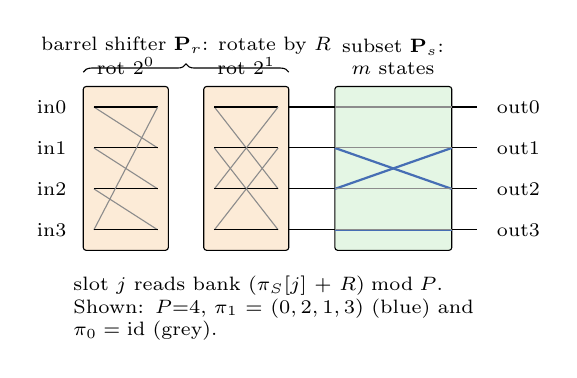
\begin{tikzpicture}[font=\scriptsize,>=Stealth,x=9mm,y=5.2mm]
  \foreach \i in {0,...,3} {
    \node[anchor=east] at (-0.25,-\i) {in\i};
    \node[anchor=west] at (5.55,-\i) {out\i};
  }
  % barrel shifter: two rotation stages (rot by 1, rot by 2)
  \foreach \s/\r in {0/1, 1/2} {
    \draw[fill=blkcomp,rounded corners=1pt] (\s*1.7-0.15,-3.5) rectangle (\s*1.7+1.05,0.5);
    \node[anchor=south] at (\s*1.7+0.45,0.55) {rot $2^{\s}$};
    \foreach \i in {0,...,3} {
      \pgfmathtruncatemacro{\j}{mod(\i+\r,4)}
      \draw[black!45] (\s*1.7,-\i) -- (\s*1.7+0.9,-\j);
      \draw (\s*1.7,-\i) -- (\s*1.7+0.9,-\i);
    }
  }
  \draw[decorate,decoration={brace,amplitude=3pt}] (-0.15,0.85) -- (2.75,0.85)
     node[midway,above=3pt]{barrel shifter $\mathbf{P}_r$: rotate by $R$};
  % subset switch: two states pi_0 = id, pi_1 = (0,2,1,3)
  \draw[fill=blkctl,rounded corners=1pt] (3.4,-3.5) rectangle (5.05,0.5);
  \node[anchor=south,align=center] at (4.22,0.55)
    {subset $\mathbf{P}_s$:\\$m$ states};
  \foreach \i in {0,...,3} \draw (2.75,-\i) -- (3.4,-\i);
  \foreach \i/\j in {0/0,1/2,2/1,3/3}
     \draw[barA,thick] (3.4,-\i) -- (5.05,-\j);
  \foreach \i in {0,...,3} \draw[black!45] (3.4,-\i) -- (5.05,-\i);
  \foreach \i in {0,...,3} \draw (5.05,-\i) -- (5.4,-\i);
  \node[anchor=north,align=left,text width=52mm] at (2.6,-3.9)
    {\scriptsize slot $j$ reads bank $(\pi_S[j]+R)\bmod P$.  Shown: $P{=}4$,
     $\pi_1 = (0,2,1,3)$ (blue) and $\pi_0 = \mathrm{id}$ (grey).};
\end{tikzpicture}
\caption{Permute--rotate switch for $P{=}4$.  A rotation network of $\log_2 P$
stages, composed with one of $m$ fixed stride permutations, replaces the
all-to-all crossbar at a cost of $\Theta(m\Pbu)$ two-input multiplexers.}
\label{fig:prs}
\end{figure}

\subsection{Sub-parallelism and packing}\label{sec:sub}

A datapath of width $2\Pbu$ would otherwise be obliged to zero-pad any transform
shorter than itself.  This is avoided by interleaving $\Psub = 2\Pbu / l$ short
transforms element-wise into a single computational vector and terminating the
recursion after $\log_2 l$ stages; independently, $\PN$ sequences are packed
depth-wise into the banked RAM.  Both quantities are runtime values and are
carried as descriptor fields (\S\ref{sec:format}).  The resulting cycle count
has the closed form
\begin{equation}
\text{cycles} \;\approx\; \frac{\PN\, N}{2\,\Psub\, \Pbe\, \Pbu}\;
             \log_2 \frac{N}{\Psub},
\label{eq:cycles}
\end{equation}
in which $N = \max(l, 2\Pbu)$ is the engine computational length and $\PN$ the
number of length-$l$ input sequences.  At the most demanding point of the
workload, 4{,}096 length-8 BL rows per branch on a $\Pbu{=}16$ engine,
sub-parallelism folds four transforms into each pass and omits two of the five
stages, requiring $6.7\times$ fewer cycles than padding.

\subsection{Bit-reversal write-back}\label{sec:brev}

Since the dataflow is decimation-in-frequency, the FFT results are produced in
bit-reversed order.  The write-back path applies $y_k = d_{\mathrm{rev}_n(k)}$
as the engine RAM is streamed to the global buffer.  Lane $a$ always reads bank
$a$, the destination bank is $\mathrm{rev}_m((a{+}u)\bmod P)$, and the
permutation completes in exactly $N/P$ cycles without conflict on either memory.
In the command set this reordering is expressed as an addressing mode of the
store path rather than as a separate instruction (\S\ref{sec:format}); for
learned BL layers it is omitted, since the output order is absorbed into the
weights of the following layer.

\subsection{The workload}\label{sec:workload}

BSPNet, used throughout in its cfg-6 configuration, classifies 32{,}768-sample
IQ records into eight modulation classes.  The computation comprises the
elementwise powers $s^2,s^4,s^6,s^8$ (Eq.~1 of~\cite{flexbe}), four $N$-point
FFTs, and then eight branches, each containing a magnitude operation, a length-8
feature expansion, and three blocks of two length-32 BL layers with a fused
LayerNorm--shortcut--ReLU--maxpool operation (``NormPool'').
Table~\ref{tab:breakdown} reports the per-module cycle budget on the
$\Pbe{\times}\Pbu = 4{\times}16$ array, totalling \CfgCycles{} cycles, or
\CfgUs\,$\mu$s at 300\,MHz.  Two structural properties of this workload shape
the architecture: the graph is static, and it contains only about one hundred
coarse operations.

\begin{table}[t]
\centering\small
\caption{cfg-6 single-inference cycle budget on the $4\times16$ BU array at
300\,MHz (from the validated Eq.~\ref{eq:cycles} model).}
\label{tab:breakdown}
\setlength{\tabcolsep}{4pt}
\begin{tabular}{@{}lrr@{}}
\toprule
module & cycles & $\mu$s \\
\midrule
\breakdownrows
\bottomrule
\end{tabular}
\end{table}

% ---------------------------------------------------------------------------
\section{Why Microcode, and at What Granularity}\label{sec:granularity}

The datapath retires $\Pbe\Pbu = 64$ butterflies per cycle.  A programmable
front end must therefore supply work at a rate of 64 butterflies per issued unit
simply to break even, and a control scheme that issued one instruction per
butterfly stage per data chunk would require hundreds of butterflies of work per
instruction to keep the pipeline occupied.  The workload, however, presents only
about one hundred coarse operations per 214\,$\mu$s inference.  The efficient
operating point is consequently well defined: the unit of issue should be the
layer, and issue should be asynchronous so that data movement is overlapped with
computation.

The choice of mechanism is further constrained in two respects.  The application
processors of the target Zynq UltraScale+ MPSoC are hard Cortex-A53 cores that
expose no custom-instruction port, so tight coupling in the RoCC style is
unavailable and control must be delivered over AXI.  Per-command AXI writes are
also costly: at approximately 0.4\,$\mu$s per posted MMIO write, the \ProgCmds{}
commands of an inference amount to some 42\,$\mu$s, or 19\% of the inference
time, before any other overhead is considered, and an interactive Python flow
increases this figure by two orders of magnitude (\S\ref{sec:eval}).  The
established response is microprogramming~\cite{wilkes1953} in its modern
accelerator form, in which the host writes a program of descriptors to memory
once and a small hardware sequencer fetches and executes
them~\cite{nvdla,vta,gemmini}.  As the command graph is static, the
steady-state host cost per inference is reduced to a single pointer update and a
single doorbell.

A further principle constrains the content of the descriptors.  The
conflict-free addressing of \S\ref{sec:sched} is a derived property of the
memory mapping, and enumerating it in software would fix it in every program.
Descriptors are therefore restricted to naming memories, transforms, and shapes,
and never a bank, a switch state, or a cycle, so that the schedule remains a
microarchitectural matter.

% ---------------------------------------------------------------------------
\section{Architecture}\label{sec:arch}

\begin{figure*}[t]
\centering
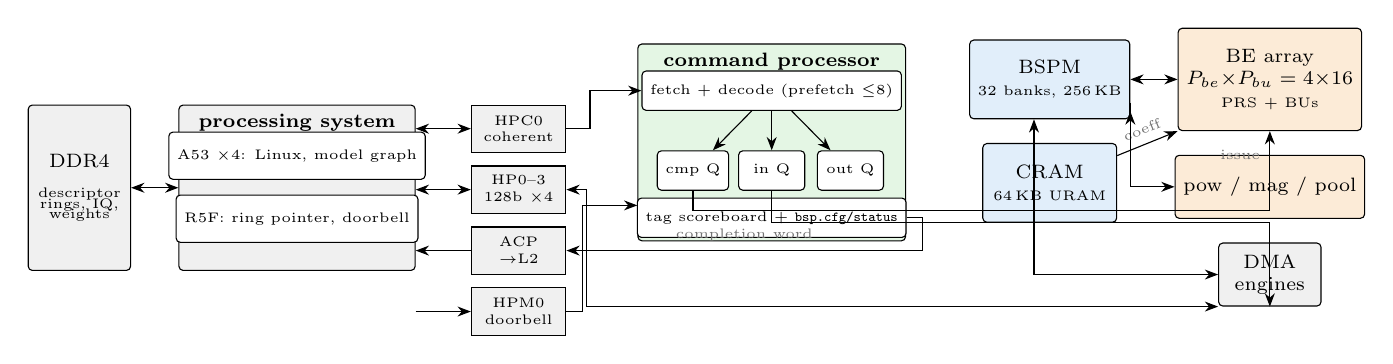
\begin{tikzpicture}[font=\scriptsize,>=Stealth,
  blk/.style={draw,rounded corners=1.5pt,minimum height=9mm,inner sep=3pt,align=center},
  port/.style={draw,fill=blkio,minimum height=6mm,inner sep=2pt,align=center,font=\tiny},
  lbl/.style={font=\tiny,text=black!55}]
  % ---- processing system ----
  \node[blk,fill=blkio,minimum width=30mm,minimum height=21mm,align=center]
     (ps) at (0,0) {};
  \node[anchor=north,font=\scriptsize\bfseries] at (ps.north) {processing system};
  \node[blk,fill=white,minimum width=24mm,minimum height=6mm,font=\tiny]
     at ($(ps.north)+(0,-6.5mm)$) (a53) {A53 $\times$4: Linux, model graph};
  \node[blk,fill=white,minimum width=24mm,minimum height=6mm,font=\tiny]
     at ($(ps.north)+(0,-14.5mm)$) (r5) {R5F: ring pointer, doorbell};
  \node[blk,fill=blkio,minimum width=13mm,minimum height=21mm,left=6mm of ps]
     (ddr) {DDR4\\[1mm]\tiny descriptor\\[-1.5mm]\tiny rings, IQ,\\[-1.5mm]\tiny weights};
  \draw[<->] (ddr) -- (ps);
  % ---- ports column ----
  \node[port,minimum width=12mm,right=7mm of ps.north east,anchor=north west]
     (hpc) {HPC0\\coherent};
  \node[port,minimum width=12mm,below=1.6mm of hpc] (hp) {HP0--3\\128b $\times$4};
  \node[port,minimum width=12mm,below=1.6mm of hp] (acp) {ACP\\$\rightarrow$L2};
  \node[port,minimum width=12mm,below=1.6mm of acp] (hpm) {HPM0\\doorbell};
  \draw[<->] (ps.east|-hpc) -- (hpc);
  \draw[<->] (ps.east|-hp) -- (hp);
  \draw[<-]  (ps.east|-acp) -- (acp);
  \draw[->]  (ps.east|-hpm) -- (hpm);
  % ---- sequencer ----
  \node[blk,fill=blkctl,minimum width=34mm,minimum height=25mm,right=9mm of hp,
        yshift=6mm] (seq) {};
  \node[anchor=north,font=\scriptsize\bfseries] at (seq.north)
     {command processor};
  \node[blk,fill=white,font=\tiny,minimum width=28mm,minimum height=5mm]
     at ($(seq.north)+(0,-6mm)$) (fetch) {fetch + decode (prefetch $\le$8)};
  \node[blk,fill=white,font=\tiny,minimum width=8.4mm,minimum height=5mm]
     at ($(seq.south)+(-10mm,9mm)$) (qc) {cmp Q};
  \node[blk,fill=white,font=\tiny,minimum width=8.4mm,minimum height=5mm]
     at ($(seq.south)+(0mm,9mm)$)  (qi) {in Q};
  \node[blk,fill=white,font=\tiny,minimum width=8.4mm,minimum height=5mm]
     at ($(seq.south)+(10mm,9mm)$) (qo) {out Q};
  \node[blk,fill=white,font=\tiny,minimum width=28mm,minimum height=5mm]
     at ($(seq.south)+(0,3mm)$) (score) {tag scoreboard + \texttt{bsp.cfg/status}};
  \draw[->] (fetch) -- (qc); \draw[->] (fetch) -- (qi); \draw[->] (fetch) -- (qo);
  \draw[->] (hpc.east) -- ++(3mm,0) |- (fetch.west);
  \draw[->] (hpm.east) -- ++(2mm,0) |- ($(seq.west)+(0,-8mm)$);
  % ---- datapath ----
  \node[blk,fill=blkmem,minimum width=17mm,minimum height=10mm,right=8mm of seq,
        yshift=8mm] (bspm) {BSPM\\ \tiny 32 banks, 256\,KB};
  \node[blk,fill=blkmem,minimum width=17mm,minimum height=10mm,below=3mm of bspm]
     (cram) {CRAM\\ \tiny 64\,KB URAM};
  \node[blk,fill=blkcomp,minimum width=20mm,minimum height=13mm,right=6mm of bspm]
     (be) {BE array\\ $\Pbe{\times}\Pbu = 4{\times}16$\\ \tiny PRS + BUs};
  \node[blk,fill=blkcomp,minimum width=20mm,minimum height=8mm,below=3mm of be]
     (glue) {pow / mag / pool};
  \node[blk,fill=blkio,minimum width=13mm,minimum height=8mm,below=3mm of glue]
     (dma) {DMA\\engines};
  \draw[<->] (bspm) -- (be);
  \draw[->] (cram) -- node[lbl,above,sloped]{coeff} (be.south west);
  \draw[<->] ($(bspm.south east)+(0,1mm)$) -- ++(0,0) |- (glue.west);
  \draw[<->] (dma.west) -| ($(bspm.south)+(-2mm,0)$);
  \draw[<->] (hp.east) -- ++(2.5mm,0) |- (dma.south west);
  \draw[->] (qc.south) -- ++(0,-2.5mm) -| node[lbl,pos=0.85,left]{issue} (be.south);
  \draw[->] (qi.south) -- ++(0,-4mm) -| (dma.south);
  \draw[->] (score.east) -- ++(2mm,0) |- node[lbl,pos=0.75,above]{completion word}
      (acp.east);
\end{tikzpicture}
\caption{System organisation on the Zynq UltraScale+ MPSoC.  The command
processor fetches 32-byte descriptors from coherent memory over HPC0, prefetching
up to a ring of them, dispatches them into per-resource queues, and retires
completions by writing a word through ACP that the host polls in the L2 cache.
Bulk IQ data and features are moved over the HP ports, and the doorbell is a
single HPM0 write per inference.}
\label{fig:system}
\end{figure*}

\subsection{System organisation}
The machine is shown in Fig.~\ref{fig:system}.  The command processor is
positioned between the AXI ports and the fixed-function datapath, and comprises
a descriptor fetch and decode unit, three shallow per-resource queues for
compute, DMA-in, and DMA-out, a tag scoreboard, and a completion writer.  The
remainder of the machine is the published engine, used without modification: the
BE array, the coefficient RAM, the banked butterfly scratchpad, and the
pointwise units.

\subsection{Architectural state}
The state that a descriptor program may name is listed in Table~\ref{tab:state}.
The butterfly scratchpad (BSPM) is addressed by logical element index, the
shift-down skew of Eq.~\ref{eq:bsm} being applied in hardware and hidden from
software.  This abstraction is central to the design, since it preserves
in-place operation and the private coefficient port, both of which are lost in a
programmable design based on a register file, while leaving the bank mapping
free to change.

\begin{table}[t]
\centering\small
\caption{Architectural state ($\Pbe{=}4$, $\Pbu{=}16$).}
\label{tab:state}
\setlength{\tabcolsep}{3.5pt}
\begin{tabular}{@{}lll@{}}
\toprule
state & size & visibility \\
\midrule
\texttt{BSPM} scratchpad & 256\,KB & logical index; skew in hardware \\
\texttt{CRAM} coefficients & 64\,KB & twiddles / BL weights, Table~4 layout \\
\texttt{bsp.cfg} & 64\,b & defaults: $l$, $\Psub$, $\PN$, Q-format \\
\texttt{bsp.status} & 64\,b & busy mask, queue depth, error, cycles \\
descriptor rings & 3.3\,KB & in DDR, fetched over HPC0 \\
tag scoreboard & 8\,b$\times$slots & microarchitectural, read via status \\
\bottomrule
\end{tabular}
\end{table}

\subsection{Sequencer microarchitecture}
The sequencer operates in three stages.  In the fetch stage, descriptors are
read over the coherent HPC0 port up to a configurable prefetch depth ahead of
retirement, bounded by the ring capacity; a depth of four to eight is shown in
\S\ref{sec:eval} to be sufficient.  In the decode stage, a descriptor is
expanded into engine control.  For \op{bs.bfly} this consists of initialising
the loop counters $(k, j, \text{seq})$, whose body is
$\mathsf{cycle\_control}$, together with the CRAM base and the arithmetic mode;
the decode reduces to a small number of field extractions.  In the dispatch
stage, the command is placed in the queue of its resource class.  Commands are
issued in program order within each resource, and a command begins only once the
tags it names have retired.  Because dependencies are stated explicitly in the
descriptor, the scoreboard is a small table of tag-to-done bits rather than an
associative structure.  Separating the queues by resource permits the input DMA
of the next inference to be fetched and started while the current inference
computes; with a single shared queue this descriptor would be held behind the
roughly one hundred compute descriptors ahead of it, and \S\ref{sec:eval}
quantifies the resulting difference.

Completion is signalled through memory rather than by interrupt.  At 214\,$\mu$s
per job the Linux interrupt latency of 5--10\,$\mu$s is significant, so the
sequencer writes a completion word through the ACP port, which allocates into
the A53 L2 cache, and the host polls it.  In the tuned configuration the
Cortex-R5F of the real-time unit owns the ring and the doorbell over the
low-latency LPD port, leaving the A53 cluster to run Linux.

\subsection{Datapath commands}
Three units are driven by the compute descriptors.  The \op{bs.bfly} descriptor
runs the engine loop of Fig.~\ref{fig:datapath} for
$\lceil \PN/\Psub \rceil \cdot (N/2\Pbu) \cdot \log_2(N/\Psub)$ cycles per
engine, so that Eq.~\ref{eq:cycles} serves directly as its latency formula.  The
\op{bs.brev} descriptor runs the write-back network of \S\ref{sec:brev} for
$N/P$ cycles; the same network serves \op{bs.store} when the \texttt{BITREV}
flag is set, so that natural-order output is obtained through an addressing mode
rather than an additional pass.  The \op{bs.pow}, \op{bs.mag}, and \op{bs.pool}
descriptors drive the pointwise units already present in the published system,
in which magnitude computation alone occupies 41\,k LUTs; treating these units
as architectural keeps the inputs of all eight branches on chip.

% ---------------------------------------------------------------------------
\section{Microcode Format}\label{sec:format}

\begin{figure}[t]
\centering
\begin{bytefield}[bitwidth=0.0255\linewidth,bitheight=4.2mm,
                  boxformatting={\centering\tiny}]{32}
\bitheader[endianness=big]{0,7,8,15,16,23,24,31}\\
\bitbox{8}{\texttt{log2\_l}} & \bitbox{8}{\texttt{mode}} &
\bitbox{8}{\texttt{flags}} & \bitbox{8}{\texttt{opcode}}\\
\bitbox{8}{\texttt{pool}} & \bitbox{8}{\texttt{stage\_hi}} &
\bitbox{8}{\texttt{stage\_lo}} & \bitbox{8}{\texttt{log2\_Psub}}\\
\bitbox{32}{\texttt{src} --- BSPM / VA source}\\
\bitbox{32}{\texttt{dst} --- BSPM / VA destination}\\
\bitbox{32}{\texttt{coeff} --- CRAM base}\\
\bitbox{32}{\texttt{count} --- elements / bytes}\\
\bitbox{32}{\texttt{P\_N} --- sequences of length $l$}\\
\bitbox{32}{\texttt{tag} --- completion / dependency token}
\end{bytefield}
\caption{The 32-byte descriptor (little endian, with word~0 at the top and
bit~0 at the right).  All shape parameters of the engine, namely $l$, $\Psub$,
$\PN$, and the stage window, are carried as operand fields.}
\label{fig:descriptor}
\end{figure}

\subsection{Descriptor layout}
Each command occupies a single 32-byte word (Fig.~\ref{fig:descriptor}),
consisting of eight single-byte control fields followed by six 32-bit operands.
This size corresponds to one beat of a 256-bit AXI read, so that a descriptor is
fetched in a single transaction, and the complete cfg-6 program occupies
\ProgBytes{} bytes, less than the first few kilobytes of one input record.

\subsection{Opcode set and semantics}
The eight opcodes, their resource classes, and their latencies in engine cycles
or transferred bytes are given in Table~\ref{tab:opcodes}.  Three conventions
account for most of the encoding.  Shapes are represented as logarithms: the
fields \texttt{log2\_l} and \texttt{log2\_Psub} render non-power-of-two shapes
unrepresentable and decode directly to shift amounts.  The stage window
\texttt{[stage\_lo, stage\_hi]} defaults to the full transform but admits
partial passes, which provide both the early termination used by
sub-parallelism and a convenient means of debugging.  Flags compose: a NormPool
block is expressed as a single \op{bs.pool} descriptor with
\texttt{LAYERNORM|SHORTCUT|RELU|MAXPOOL}, and BL layers fuse their activation by
setting \texttt{RELU} on \op{bs.bfly}.

\begin{table}[t]
\centering\small
\caption{Opcode set.  $C(\cdot)$ abbreviates Eq.~\ref{eq:cycles}.}
\label{tab:opcodes}
\setlength{\tabcolsep}{3pt}
\begin{tabular}{@{}llll@{}}
\toprule
opcode & class & semantics & latency \\
\midrule
\op{bs.load}  & dma-in  & mem $\to$ BSPM & bytes/BW \\
\op{bs.wload} & dma-in  & mem $\to$ CRAM & bytes/BW \\
\op{bs.store} & dma-out & BSPM $\to$ mem; \texttt{BITREV}, \texttt{MAG} & bytes/BW \\
\op{bs.bfly}  & compute & $\PN$ transforms, len $l$; FFT/IFFT/ & $C(l,\Psub,\PN)$ \\
              &         & \quad BL/BL\_EXPAND; \texttt{RELU} & \\
\op{bs.brev}  & compute & write-back reversal pass & $\PN N/P$ \\
\op{bs.pow}   & compute & $s^p$, $p \in \texttt{mode}$ & $N/128$ \\
\op{bs.mag}   & compute & $|x|$; \texttt{NORMALISE} & $N/128$ \\
\op{bs.pool}  & compute & LN/shortcut/ReLU/maxpool$_f$ & rows$/8$ \\
\bottomrule
\end{tabular}
\end{table}

\subsection{Encodings}
Five encoded descriptors from the worked example are shown in
Table~\ref{tab:hex}, exactly as emitted by the assembler in the accompanying
artifact.  The second row illustrates the density of the encoding: the entire
four-FFT feature-extraction stage, comprising \HeadlineCycles{} datapath cycles,
is represented by a single word with \texttt{log2\_l}=15, \texttt{P\_N}=4, and
\texttt{stage\_hi}=14.

\begin{table*}[t]
\centering\scriptsize
\caption{Encoded descriptors (eight little-endian words each; words 0--3 on
the first line, 4--7 on the second).}
\label{tab:hex}
\setlength{\tabcolsep}{4pt}
\begin{tabular}{@{}llp{5.4cm}@{}}
\toprule
descriptor & encoding (words 0..7) & meaning \\
\midrule
\programhexrows
\bottomrule
\end{tabular}
\end{table*}

\subsection{Decode into engine control}
The decode of \op{bs.bfly} is intentionally lightweight.  The hardware derives
$N = \max(2^{\texttt{log2\_l}},\,2\Pbu)$ and, when $l < 2\Pbu$, the interleave
factor $\Psub = 2\Pbu/l$; it distributes \texttt{P\_N} across the $\Pbe$
engines; and it initialises three counters, for the stage $k$, the cycle $j$,
and the packed sequence.  The per-cycle work is then given entirely by the
closed form of \S\ref{sec:sched}: an insert-zero network positioned by the
stage-constant hole bit produces $\mathbf{I}^i$, a population count already
present in the bsm datapath produces $R^i$, and $S^i$ is obtained from a
comparison of $h$ with $m$.  No field of the descriptor constrains this
machinery.  The schedule is derived at decode time from the same two-regime rule
that the memory mapping imposes, and could be re-derived under a different rule
without any change to software.

% ---------------------------------------------------------------------------
\section{Worked Example}\label{sec:worked}

The machine is examined at two scales: a single \op{bs.bfly} descriptor
executing a 16-point FFT, for which every cycle may be tabulated, and the
complete cfg-6 inference, in which the behaviour of interest is the overlap of
computation with data movement.

\subsection{One descriptor, cycle by cycle}
A small engine is configured with $\Pbu = 2$ ($P = 4$ banks, $m = 2$), and the
descriptor
\begin{center}\footnotesize
\op{bs.bfly}\{\texttt{mode}=FFT, \texttt{log2\_l}=4, \texttt{P\_N}=1,
\texttt{stage\_hi}=3\}
\end{center}
is issued on input $x_0..x_{15}$ resident in BSPM under the layout of
Fig.~\ref{fig:memory}.  Decode yields $N{=}16$, $\Psub{=}1$, and four stages of
$N/2\Pbu = \WeCPS$ cycles.  The complete control trace emitted by
$\mathsf{cycle\_control}$ is given in Table~\ref{tab:trace}, and the data
movement of the first cycle is drawn in Fig.~\ref{fig:cycle}.  Three properties
may be verified against the table.

\begin{figure}[t]
\centering
\resizebox{0.97\linewidth}{!}{%
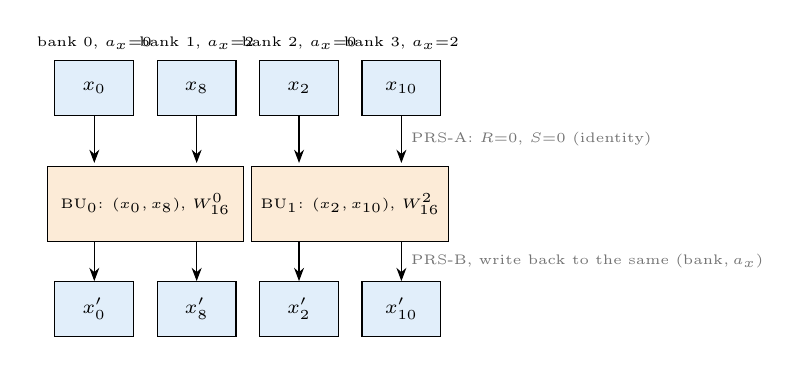
\begin{tikzpicture}[font=\scriptsize,>=Stealth,x=1mm,y=1mm]
  % banks
  \foreach \b/\e/\d in {0/x_{0}/0, 1/x_{8}/2, 2/x_{2}/0, 3/x_{10}/2} {
    \draw[fill=blkmem] (\b*13,0) rectangle (\b*13+10,7);
    \node at (\b*13+5,3.5) {$\e$};
    \node[anchor=south,font=\tiny] at (\b*13+5,7.2) {bank \b, $a_x{=}\d$};
  }
  % PRS identity (R=0,S=0)
  \foreach \b in {0,...,3} \draw[->] (\b*13+5,0) -- (\b*13+5,-6);
  \node[anchor=west,font=\tiny,text=black!55] at (44,-3)
     {PRS-A: $R{=}0$, $S{=}0$ (identity)};
  % BU boxes
  \draw[fill=blkcomp] (-1,-16) rectangle (24,-6.5);
  \node[font=\tiny] at (11.5,-11.2)
     {BU$_0$: $(x_0,x_8)$, $W_{16}^{0}$};
  \draw[fill=blkcomp] (25,-16) rectangle (50,-6.5);
  \node[font=\tiny] at (37.5,-11.2)
     {BU$_1$: $(x_2,x_{10})$, $W_{16}^{2}$};
  % outputs
  \foreach \b in {0,...,3} \draw[->] (\b*13+5,-16) -- (\b*13+5,-21);
  \node[anchor=west,font=\tiny,text=black!55] at (44,-18.5)
     {PRS-B, write back to the same $(\mathrm{bank},a_x)$};
  \foreach \b/\e in {0/x'_{0}, 1/x'_{8}, 2/x'_{2}, 3/x'_{10}} {
    \draw[fill=blkmem] (\b*13,-28) rectangle (\b*13+10,-21);
    \node at (\b*13+5,-24.5) {$\e$};
  }
\end{tikzpicture}}
\caption{Stage $k{=}0$, cycle $j{=}0$ of the worked example.  With hole bit
$h{=}3$, the pairs $(0,8)$ and $(2,10)$ span rows 0 and 2.  The banks
$\bsm = (0,1,2,3)$ are distinct, the address vector supplies a different depth
per bank, $(0,2,0,2)$, and the permutation is a pure rotation by
$R{=}\mathrm{pc}(0){+}e{=}0$, so that $S{=}0$.  The coefficient addresses
$(0,2)$ select $W_{16}^{0}$ and $W_{16}^{2}$.}
\label{fig:cycle}
\end{figure}

\begin{table*}[t]
\centering\footnotesize
\caption{Complete control trace of the worked example: 16-point FFT,
$\Pbu{=}2$.  Each row gives, for one cycle, the index vector $\mathbf{I}^i$ in
slot order, its banks $\bsm(\mathbf{I}^i)$, which are always a permutation of
$0..3$, the per-bank address vector $\mathrm{Addr}^i$, the PRS rotation $R^i$
and subset state $S^i$, and the coefficient addresses of the two butterflies.
Stages 0 and 1 are in the two-row regime ($h \ge m$, $S{=}0$, a pure rotation);
stage 2 is in the in-row regime with the stride permutation ($S{=}1$); and stage
3 is in-row with adjacent pairs ($S{=}0$).}
\label{tab:trace}
\setlength{\tabcolsep}{5.5pt}
\begin{tabular}{@{}ccccccccc@{}}
\toprule
$k$ & $h$ & $j$ & $\mathbf{I}^i$ (slots $0..3$) & $\bsm(\mathbf{I}^i)$ &
$\mathrm{Addr}^i$ (banks $0..3$) & $R^i$ & $S^i$ & coeff \\
\midrule
\tracetablerows
\bottomrule
\end{tabular}
\end{table*}

\begin{itemize}\setlength\itemsep{1pt}
\item Conflict freedom.  Every $\bsm$ column is a permutation of $(0,1,2,3)$,
      without exception across the sixteen cycles.  The address column indicates
      why a per-bank address vector is required in place of a single shared
      address: in the two-row regime, half of the banks are read at a different
      depth.
\item Switch economy.  Over all \WeCycles{} cycles the subset state assumes only
      the values $\{0,1\}$, that is $h$ when $h<m$, which is two of the $m{=}2$
      available states, while the rotation $R^i$ follows $\mathrm{pc}(H)+e$.
      This behaviour is what justifies the use of the PRS in place of a
      crossbar.
\item Latency.  The four stages of \WeCPS{} cycles give \WeCycles{} butterfly
      cycles, in exact agreement with Eq.~\ref{eq:cycles}, together with
      \WeBrev{} write-back cycles when the result is stored with the
      \texttt{BITREV} flag.  The simulator executes this trace and agrees with
      \texttt{numpy.fft} to within $10^{-15}$.
\end{itemize}

\subsection{A complete inference}
The head of the cfg-6 program is listed in Table~\ref{tab:program}.  The program
comprises \ProgCmds{} descriptors---\ProgDmaIn{} load, \ProgCompute{} compute,
and \ProgDmaOut{} store, in \ProgBytes{} bytes---whose dependency structure is
the directed acyclic graph of Fig.~\ref{fig:dag}.  The program is constructed by
the host once, after which each inference requires only a single pointer update
and a single doorbell.

\begin{table}[t]
\centering\footnotesize
\caption{Head and tail of the cfg-6 descriptor program.}
\label{tab:program}
\setlength{\tabcolsep}{2.6pt}
\begin{tabular}{@{}rllllr@{}}
\toprule
tag & opcode & operand summary & class & cost & deps \\
\midrule
\programheadrows
\bottomrule
\end{tabular}
\end{table}

\begin{figure}[t]
\centering
\resizebox{\linewidth}{!}{%
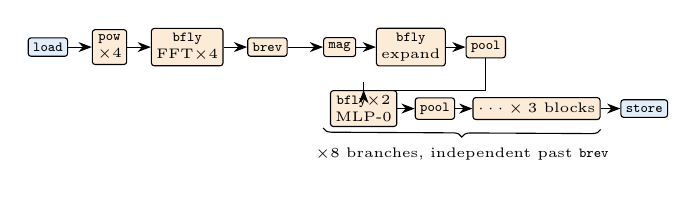
\begin{tikzpicture}[font=\tiny,>=Stealth,node distance=2.2mm,
  n/.style={draw,rounded corners=1pt,inner sep=1.8pt,align=center,fill=blkcomp},
  d/.style={draw,rounded corners=1pt,inner sep=1.8pt,align=center,fill=blkmem}]
  \node[d] (load) {\op{load}};
  \node[n,right=3mm of load] (pow) {\op{pow}\\$\times4$};
  \node[n,right=3mm of pow] (fft) {\op{bfly}\\FFT$\times$4};
  \node[n,right=3mm of fft] (brev) {\op{brev}};
  \node[n,right=4.5mm of brev] (mag) {\op{mag}};
  \node[n,right=2.5mm of mag] (exp) {\op{bfly}\\expand};
  \node[n,right=2.5mm of exp] (p0) {\op{pool}};
  \node[n,below=3mm of exp,xshift=-6mm] (m0) {\op{bfly}$\times$2\\MLP-0};
  \node[n,right=2.2mm of m0] (n0) {\op{pool}};
  \node[n,right=2.2mm of n0] (m1) {$\cdots\times3$ blocks};
  \node[d,right=2.5mm of m1] (store) {\op{store}};
  \draw[->] (load) -- (pow); \draw[->] (pow) -- (fft);
  \draw[->] (fft) -- (brev); \draw[->] (brev) -- (mag);
  \draw[->] (mag) -- (exp); \draw[->] (exp) -- (p0);
  \draw[->] (p0.south) |- (m0.east|-m0.north) -| (m0.north);
  \draw[->] (m0) -- (n0); \draw[->] (n0) -- (m1); \draw[->] (m1) -- (store);
  \draw[decorate,decoration={brace,mirror,amplitude=3pt}]
    ($(mag.south west)+(0,-9mm)$) -- ($(m1.south east)+(0,-1.2mm)$)
    node[midway,below=3.5pt]{$\times$8 branches, independent past \op{brev}};
\end{tikzpicture}}
\caption{Dependency structure of the cfg-6 program.  The eight branches are
independent following the write-back, so that computation does not starve, and
the final store joins the tails of all branches.}
\label{fig:dag}
\end{figure}

The model's execution timeline for two consecutive inferences on the tuned
platform is shown in Fig.~\ref{fig:timeline}.  The input DMA of inference~1,
shown in orange on the DMA-in lane, is fetched from its own queue and completes
entirely within the computation of inference~0; this overlap is precisely what a
shared descriptor queue would prevent.  The steady-state cost per inference is
consequently \TimelineTwoPerInf\,$\mu$s, against a datapath time of
\CfgUs\,$\mu$s.  The remaining difference is dominated by the 128\,KB landing
time of the first record, which cannot be overlapped at a batch size of one
unless the radio front end is streamed directly into BSPM.

\begin{figure*}[t]
\centering
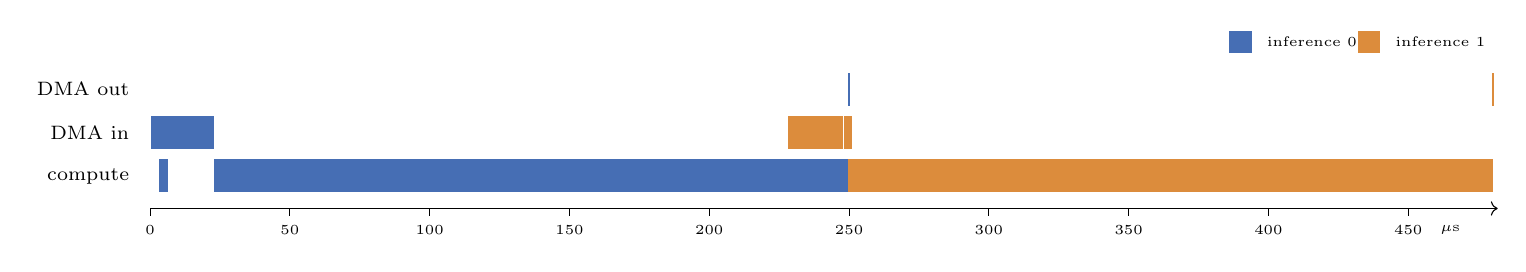
\begin{tikzpicture}[x=0.0355cm,y=0.55cm,font=\scriptsize]
  % lanes: 0=compute 1=dma_in 2=dma_out; x in us
\fill[barA] (0.20,1.12) rectangle (3.01,1.88);
\fill[barA] (3.01,1.12) rectangle (5.82,1.88);
\fill[barA] (5.82,1.12) rectangle (8.63,1.88);
\fill[barA] (8.63,1.12) rectangle (11.44,1.88);
\fill[barA] (11.44,1.12) rectangle (14.25,1.88);
\fill[barA] (14.25,1.12) rectangle (17.06,1.88);
\fill[barA] (17.06,1.12) rectangle (19.87,1.88);
\fill[barA] (19.87,1.12) rectangle (22.68,1.88);
\fill[barA] (3.01,0.12) rectangle (3.86,0.88);
\fill[barA] (3.86,0.12) rectangle (4.72,0.88);
\fill[barA] (4.72,0.12) rectangle (5.57,0.88);
\fill[barA] (5.57,0.12) rectangle (6.42,0.88);
\fill[barA] (22.68,0.12) rectangle (73.88,0.88);
\fill[barA] (73.88,0.12) rectangle (77.29,0.88);
\fill[barA] (77.29,0.12) rectangle (78.15,0.88);
\fill[barA] (78.15,0.12) rectangle (88.39,0.88);
\fill[barA] (88.39,0.12) rectangle (88.60,0.88);
\fill[barA] (88.60,0.12) rectangle (92.87,0.88);
\fill[barA] (92.87,0.12) rectangle (97.13,0.88);
\fill[barA] (97.13,0.12) rectangle (97.56,0.88);
\fill[barA] (97.56,0.12) rectangle (98.09,0.88);
\fill[barA] (98.09,0.12) rectangle (98.63,0.88);
\fill[barA] (98.63,0.12) rectangle (98.78,0.88);
\fill[barA] (98.68,0.12) rectangle (98.83,0.88);
\fill[barA] (98.75,0.12) rectangle (98.90,0.88);
\fill[barA] (98.81,0.12) rectangle (98.96,0.88);
\fill[barA] (98.84,0.12) rectangle (99.69,0.88);
\fill[barA] (99.69,0.12) rectangle (109.93,0.88);
\fill[barA] (109.93,0.12) rectangle (110.15,0.88);
\fill[barA] (110.15,0.12) rectangle (114.41,0.88);
\fill[barA] (114.41,0.12) rectangle (118.68,0.88);
\fill[barA] (118.68,0.12) rectangle (119.11,0.88);
\fill[barA] (119.11,0.12) rectangle (119.64,0.88);
\fill[barA] (119.64,0.12) rectangle (120.17,0.88);
\fill[barA] (120.17,0.12) rectangle (120.32,0.88);
\fill[barA] (120.23,0.12) rectangle (120.38,0.88);
\fill[barA] (120.29,0.12) rectangle (120.44,0.88);
\fill[barA] (120.36,0.12) rectangle (120.51,0.88);
\fill[barA] (120.39,0.12) rectangle (121.24,0.88);
\fill[barA] (121.24,0.12) rectangle (131.48,0.88);
\fill[barA] (131.48,0.12) rectangle (131.69,0.88);
\fill[barA] (131.69,0.12) rectangle (135.96,0.88);
\fill[barA] (135.96,0.12) rectangle (140.23,0.88);
\fill[barA] (140.23,0.12) rectangle (140.65,0.88);
\fill[barA] (140.65,0.12) rectangle (141.19,0.88);
\fill[barA] (141.19,0.12) rectangle (141.72,0.88);
\fill[barA] (141.72,0.12) rectangle (141.87,0.88);
\fill[barA] (141.77,0.12) rectangle (141.92,0.88);
\fill[barA] (141.84,0.12) rectangle (141.99,0.88);
\fill[barA] (141.91,0.12) rectangle (142.06,0.88);
\fill[barA] (141.93,0.12) rectangle (142.79,0.88);
\fill[barA] (142.79,0.12) rectangle (153.03,0.88);
\fill[barA] (153.03,0.12) rectangle (153.24,0.88);
\fill[barA] (153.24,0.12) rectangle (157.51,0.88);
\fill[barA] (157.51,0.12) rectangle (161.77,0.88);
\fill[barA] (161.77,0.12) rectangle (162.20,0.88);
\fill[barA] (162.20,0.12) rectangle (162.73,0.88);
\fill[barA] (162.73,0.12) rectangle (163.27,0.88);
\fill[barA] (163.27,0.12) rectangle (163.42,0.88);
\fill[barA] (163.32,0.12) rectangle (163.47,0.88);
\fill[barA] (163.39,0.12) rectangle (163.54,0.88);
\fill[barA] (163.45,0.12) rectangle (163.60,0.88);
\fill[barA] (163.48,0.12) rectangle (164.33,0.88);
\fill[barA] (164.33,0.12) rectangle (174.57,0.88);
\fill[barA] (174.57,0.12) rectangle (174.79,0.88);
\fill[barA] (174.79,0.12) rectangle (179.05,0.88);
\fill[barA] (179.05,0.12) rectangle (183.32,0.88);
\fill[barA] (183.32,0.12) rectangle (183.75,0.88);
\fill[barA] (183.75,0.12) rectangle (184.28,0.88);
\fill[barA] (184.28,0.12) rectangle (184.81,0.88);
\fill[barA] (184.81,0.12) rectangle (184.96,0.88);
\fill[barA] (184.87,0.12) rectangle (185.02,0.88);
\fill[barA] (184.93,0.12) rectangle (185.08,0.88);
\fill[barA] (185.00,0.12) rectangle (185.15,0.88);
\fill[barA] (185.03,0.12) rectangle (185.88,0.88);
\fill[barA] (185.88,0.12) rectangle (196.12,0.88);
\fill[barA] (196.12,0.12) rectangle (196.33,0.88);
\fill[barA] (196.33,0.12) rectangle (200.60,0.88);
\fill[barA] (200.60,0.12) rectangle (204.87,0.88);
\fill[barA] (204.87,0.12) rectangle (205.29,0.88);
\fill[barA] (205.29,0.12) rectangle (205.83,0.88);
\fill[barA] (205.83,0.12) rectangle (206.36,0.88);
\fill[barA] (206.36,0.12) rectangle (206.51,0.88);
\fill[barA] (206.41,0.12) rectangle (206.56,0.88);
\fill[barA] (206.48,0.12) rectangle (206.63,0.88);
\fill[barA] (206.55,0.12) rectangle (206.70,0.88);
\fill[barA] (206.57,0.12) rectangle (207.43,0.88);
\fill[barA] (207.43,0.12) rectangle (217.67,0.88);
\fill[barA] (217.67,0.12) rectangle (217.88,0.88);
\fill[barA] (217.88,0.12) rectangle (222.15,0.88);
\fill[barA] (222.15,0.12) rectangle (226.41,0.88);
\fill[barA] (226.41,0.12) rectangle (226.84,0.88);
\fill[barA] (226.84,0.12) rectangle (227.37,0.88);
\fill[barA] (227.37,0.12) rectangle (227.91,0.88);
\fill[barA] (227.91,0.12) rectangle (228.06,0.88);
\fill[barA] (227.96,0.12) rectangle (228.11,0.88);
\fill[barA] (228.03,0.12) rectangle (228.18,0.88);
\fill[barA] (228.09,0.12) rectangle (228.24,0.88);
\fill[barA] (228.12,0.12) rectangle (228.97,0.88);
\fill[barA] (228.97,0.12) rectangle (239.21,0.88);
\fill[barA] (239.21,0.12) rectangle (239.43,0.88);
\fill[barA] (239.43,0.12) rectangle (243.69,0.88);
\fill[barA] (243.69,0.12) rectangle (247.96,0.88);
\fill[barA] (247.96,0.12) rectangle (248.39,0.88);
\fill[barA] (248.39,0.12) rectangle (248.92,0.88);
\fill[barA] (248.92,0.12) rectangle (249.45,0.88);
\fill[barA] (249.45,0.12) rectangle (249.60,0.88);
\fill[barA] (249.51,0.12) rectangle (249.66,0.88);
\fill[barA] (249.57,0.12) rectangle (249.72,0.88);
\fill[barA] (249.64,0.12) rectangle (249.79,0.88);
\fill[barA] (249.67,2.12) rectangle (250.24,2.88);
\fill[barB] (228.21,1.12) rectangle (231.02,1.88);
\fill[barB] (231.02,1.12) rectangle (233.83,1.88);
\fill[barB] (233.83,1.12) rectangle (236.64,1.88);
\fill[barB] (236.64,1.12) rectangle (239.45,1.88);
\fill[barB] (239.45,1.12) rectangle (242.26,1.88);
\fill[barB] (242.26,1.12) rectangle (245.07,1.88);
\fill[barB] (245.07,1.12) rectangle (247.88,1.88);
\fill[barB] (248.06,1.12) rectangle (250.87,1.88);
\fill[barB] (249.67,0.12) rectangle (250.52,0.88);
\fill[barB] (250.52,0.12) rectangle (251.37,0.88);
\fill[barB] (251.37,0.12) rectangle (252.23,0.88);
\fill[barB] (252.23,0.12) rectangle (253.08,0.88);
\fill[barB] (253.08,0.12) rectangle (304.28,0.88);
\fill[barB] (304.28,0.12) rectangle (307.69,0.88);
\fill[barB] (307.69,0.12) rectangle (308.55,0.88);
\fill[barB] (308.55,0.12) rectangle (318.79,0.88);
\fill[barB] (318.79,0.12) rectangle (319.00,0.88);
\fill[barB] (319.00,0.12) rectangle (323.27,0.88);
\fill[barB] (323.27,0.12) rectangle (327.53,0.88);
\fill[barB] (327.53,0.12) rectangle (327.96,0.88);
\fill[barB] (327.96,0.12) rectangle (328.49,0.88);
\fill[barB] (328.49,0.12) rectangle (329.03,0.88);
\fill[barB] (329.03,0.12) rectangle (329.18,0.88);
\fill[barB] (329.08,0.12) rectangle (329.23,0.88);
\fill[barB] (329.15,0.12) rectangle (329.30,0.88);
\fill[barB] (329.21,0.12) rectangle (329.36,0.88);
\fill[barB] (329.24,0.12) rectangle (330.09,0.88);
\fill[barB] (330.09,0.12) rectangle (340.33,0.88);
\fill[barB] (340.33,0.12) rectangle (340.55,0.88);
\fill[barB] (340.55,0.12) rectangle (344.81,0.88);
\fill[barB] (344.81,0.12) rectangle (349.08,0.88);
\fill[barB] (349.08,0.12) rectangle (349.51,0.88);
\fill[barB] (349.51,0.12) rectangle (350.04,0.88);
\fill[barB] (350.04,0.12) rectangle (350.57,0.88);
\fill[barB] (350.57,0.12) rectangle (350.72,0.88);
\fill[barB] (350.63,0.12) rectangle (350.78,0.88);
\fill[barB] (350.69,0.12) rectangle (350.84,0.88);
\fill[barB] (350.76,0.12) rectangle (350.91,0.88);
\fill[barB] (350.79,0.12) rectangle (351.64,0.88);
\fill[barB] (351.64,0.12) rectangle (361.88,0.88);
\fill[barB] (361.88,0.12) rectangle (362.09,0.88);
\fill[barB] (362.09,0.12) rectangle (366.36,0.88);
\fill[barB] (366.36,0.12) rectangle (370.63,0.88);
\fill[barB] (370.63,0.12) rectangle (371.05,0.88);
\fill[barB] (371.05,0.12) rectangle (371.59,0.88);
\fill[barB] (371.59,0.12) rectangle (372.12,0.88);
\fill[barB] (372.12,0.12) rectangle (372.27,0.88);
\fill[barB] (372.17,0.12) rectangle (372.32,0.88);
\fill[barB] (372.24,0.12) rectangle (372.39,0.88);
\fill[barB] (372.31,0.12) rectangle (372.46,0.88);
\fill[barB] (372.33,0.12) rectangle (373.19,0.88);
\fill[barB] (373.19,0.12) rectangle (383.43,0.88);
\fill[barB] (383.43,0.12) rectangle (383.64,0.88);
\fill[barB] (383.64,0.12) rectangle (387.91,0.88);
\fill[barB] (387.91,0.12) rectangle (392.17,0.88);
\fill[barB] (392.17,0.12) rectangle (392.60,0.88);
\fill[barB] (392.60,0.12) rectangle (393.13,0.88);
\fill[barB] (393.13,0.12) rectangle (393.67,0.88);
\fill[barB] (393.67,0.12) rectangle (393.82,0.88);
\fill[barB] (393.72,0.12) rectangle (393.87,0.88);
\fill[barB] (393.79,0.12) rectangle (393.94,0.88);
\fill[barB] (393.85,0.12) rectangle (394.00,0.88);
\fill[barB] (393.88,0.12) rectangle (394.73,0.88);
\fill[barB] (394.73,0.12) rectangle (404.97,0.88);
\fill[barB] (404.97,0.12) rectangle (405.19,0.88);
\fill[barB] (405.19,0.12) rectangle (409.45,0.88);
\fill[barB] (409.45,0.12) rectangle (413.72,0.88);
\fill[barB] (413.72,0.12) rectangle (414.15,0.88);
\fill[barB] (414.15,0.12) rectangle (414.68,0.88);
\fill[barB] (414.68,0.12) rectangle (415.21,0.88);
\fill[barB] (415.21,0.12) rectangle (415.36,0.88);
\fill[barB] (415.27,0.12) rectangle (415.42,0.88);
\fill[barB] (415.33,0.12) rectangle (415.48,0.88);
\fill[barB] (415.40,0.12) rectangle (415.55,0.88);
\fill[barB] (415.43,0.12) rectangle (416.28,0.88);
\fill[barB] (416.28,0.12) rectangle (426.52,0.88);
\fill[barB] (426.52,0.12) rectangle (426.73,0.88);
\fill[barB] (426.73,0.12) rectangle (431.00,0.88);
\fill[barB] (431.00,0.12) rectangle (435.27,0.88);
\fill[barB] (435.27,0.12) rectangle (435.69,0.88);
\fill[barB] (435.69,0.12) rectangle (436.23,0.88);
\fill[barB] (436.23,0.12) rectangle (436.76,0.88);
\fill[barB] (436.76,0.12) rectangle (436.91,0.88);
\fill[barB] (436.81,0.12) rectangle (436.96,0.88);
\fill[barB] (436.88,0.12) rectangle (437.03,0.88);
\fill[barB] (436.95,0.12) rectangle (437.10,0.88);
\fill[barB] (436.97,0.12) rectangle (437.83,0.88);
\fill[barB] (437.83,0.12) rectangle (448.07,0.88);
\fill[barB] (448.07,0.12) rectangle (448.28,0.88);
\fill[barB] (448.28,0.12) rectangle (452.55,0.88);
\fill[barB] (452.55,0.12) rectangle (456.81,0.88);
\fill[barB] (456.81,0.12) rectangle (457.24,0.88);
\fill[barB] (457.24,0.12) rectangle (457.77,0.88);
\fill[barB] (457.77,0.12) rectangle (458.31,0.88);
\fill[barB] (458.31,0.12) rectangle (458.46,0.88);
\fill[barB] (458.36,0.12) rectangle (458.51,0.88);
\fill[barB] (458.43,0.12) rectangle (458.58,0.88);
\fill[barB] (458.49,0.12) rectangle (458.64,0.88);
\fill[barB] (458.52,0.12) rectangle (459.37,0.88);
\fill[barB] (459.37,0.12) rectangle (469.61,0.88);
\fill[barB] (469.61,0.12) rectangle (469.83,0.88);
\fill[barB] (469.83,0.12) rectangle (474.09,0.88);
\fill[barB] (474.09,0.12) rectangle (478.36,0.88);
\fill[barB] (478.36,0.12) rectangle (478.79,0.88);
\fill[barB] (478.79,0.12) rectangle (479.32,0.88);
\fill[barB] (479.32,0.12) rectangle (479.85,0.88);
\fill[barB] (479.85,0.12) rectangle (480.00,0.88);
\fill[barB] (479.91,0.12) rectangle (480.06,0.88);
\fill[barB] (479.97,0.12) rectangle (480.12,0.88);
\fill[barB] (480.04,0.12) rectangle (480.19,0.88);
\fill[barB] (480.07,2.12) rectangle (480.64,2.88);

  \foreach \y/\l in {0/compute, 1/DMA in, 2/DMA out}
     \node[anchor=east] at (-4,\y+0.5) {\l};
  \draw[->] (0,-0.25) -- (482,-0.25);
  \foreach \x in {0,50,...,450} {
     \draw (\x,-0.25) -- (\x,-0.42) node[below,font=\tiny] {\x};
  }
  \node[font=\tiny] at (465,-0.75) {$\mu$s};
  \fill[barA] (386,3.35) rectangle +(8,0.5);
  \node[anchor=west,font=\tiny] at (396,3.6) {inference 0};
  \fill[barB] (432,3.35) rectangle +(8,0.5);
  \node[anchor=west,font=\tiny] at (442,3.6) {inference 1};
\end{tikzpicture}
\caption{Modelled execution timeline for two inferences on the tuned platform,
which uses per-resource queues, streamed input, and an R5-driven ring.  The
input transfer of inference~1 overlaps the computation of inference~0, and the
compute lane runs essentially without gaps.  The end-to-end time is
\TimelineEnd\,$\mu$s, or \TimelineTwoPerInf\,$\mu$s per inference.}
\label{fig:timeline}
\end{figure*}

\subsection{Host code}
The steady-state host code is given in full below.
\begin{lstlisting}
/* init, once: */
ring = build_cfg6_program(weights);   /* 104 x 32 B  */
flush(ring);                          /* to coherent DDR */

/* per inference: */
ring[0].src = iq_record;              /* one pointer   */
flush(&ring[0]);
mmio_write(DOORBELL, ring_pa);        /* one AXI write */
while (!completion_word) ;            /* polls in L2   */
\end{lstlisting}

% ---------------------------------------------------------------------------
\section{Evaluation}\label{sec:eval}

\subsection{Methodology}
The results are obtained from a cycle-level model validated at three levels.  At
the engine level, the model executes the dataflow directly, using banked memory
with per-cycle conflict checking, the PRS, and general $2{\times}2$ butterflies;
it agrees with \texttt{numpy.fft} to within $10^{-13}$ across transform sizes,
sub-parallel modes, and $\PN$ packing, its measured cycle counts equal
Eq.~\ref{eq:cycles}, and its Q1.15 arithmetic attains \SqnrDb\,dB SQNR at
$N{=}1024$.  At the workload level, Eq.~\ref{eq:cycles} is applied to each
BSPNet module (Table~\ref{tab:breakdown}).  At the sequencer level, an
event-driven model of fetch, queues, DMA, and completion is used, whose only
assumptions are the processing-system latencies of Table~\ref{tab:assume}; the
timeline of Fig.~\ref{fig:timeline} is produced as its trace output.  A suite of
49 tests checks every architectural property claimed in
\S\ref{sec:engine}--\S\ref{sec:format}, including the encode and decode of
descriptors.

\begin{table}[t]
\centering\small
\caption{Processing-system timing assumptions, collected in a single dataclass
in the artifact.}
\label{tab:assume}
\setlength{\tabcolsep}{4pt}
\begin{tabular}{@{}lll@{}}
\toprule
parameter & value & confidence \\
\midrule
posted MMIO write & 0.40\,$\mu$s & medium \\
descriptor fetch (HPC0) & 0.15\,$\mu$s & medium \\
Python per-transfer cost & 25\,$\mu$s & soft; conclusion holds 5--50 \\
completion poll via ACP & 0.20\,$\mu$s & medium \\
DDR4 sustained & 6.4\,GB/s & conservative; 10\% utilised \\
sequencer LUTs & $3\text{k}+40/\text{slot}$ & rough; $10\times$ off is still small \\
\bottomrule
\end{tabular}
\end{table}

\subsection{Issue mechanism}
The principal result is given in Table~\ref{tab:platforms}.  Per-descriptor MMIO
already falls within \MmioOvh\% of the datapath, a static ring within
\StaticOvh\%, and the tuned configuration within \TunedOvh\%.  The interactive
Python flow used to benchmark the published system, by contrast, is bound by the
host: the \ProgCmds{} commands, each incurring an interpreter round trip, yield
\PynqUs\,$\mu$s and only \PynqSps{} samples per second.  The consequence for the
published measurements is direct.  Most of the gap between the measured and peak
throughput curves is attributable to processing-system software and is
recoverable with no change to the programmable logic beyond the \SeqLut-LUT
sequencer.

\begin{table}[t]
\centering\small
\caption{cfg-6 single-batch inference by issue mechanism
(datapath alone: \CfgUs\,$\mu$s).}
\label{tab:platforms}
\setlength{\tabcolsep}{3pt}
\begin{tabular}{@{}lrrrl@{}}
\toprule
mechanism & $\mu$s & ovh.\,\% & samp/s & bound by \\
\midrule
\platformrows
\bottomrule
\end{tabular}
\end{table}

\subsection{Queueing behaviour}
Prefetch depth is swept in Fig.~\ref{fig:prefetch}.  A depth of four to eight
descriptors is sufficient, since the compute commands are long relative to the
0.15\,$\mu$s fetch.  Batch size is swept in Fig.~\ref{fig:batch}.  The
shared-ring configuration reaches a plateau early, because the input descriptor
of the next inference is held behind the compute descriptors of the current one,
whereas per-resource queues allow the DMA to proceed ahead and reach
\TunedBatchTenSps{} samples per second at a batch size of ten, or
\TunedBatchTenPct\% of the \PeakSps-samples-per-second datapath peak.  This
effect is not visible to a bandwidth analysis, as the link is never the binding
constraint: \InKB\,KB in and \OutKB\,KB out per \CfgMs\,ms amount to
\LinkNeed\,GB/s of the \LinkHave{} available, or \LinkPct\%, so that a single HP
port would suffice and the four ports of Fig.~\ref{fig:system} serve only to
overlap bursts rather than to raise throughput.

\begin{figure}[t]
\centering
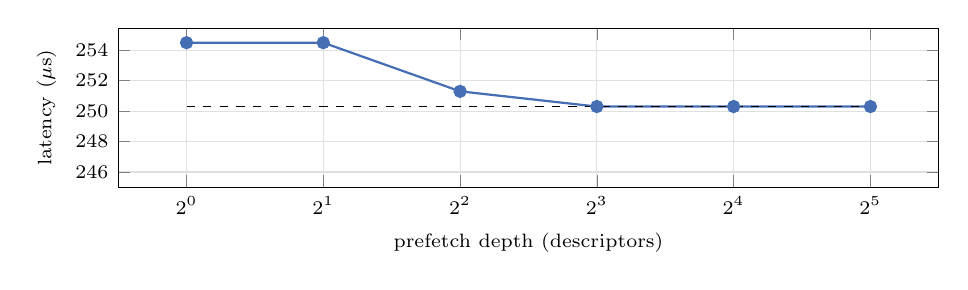
\begin{tikzpicture}
\begin{axis}[width=0.99\linewidth,height=3.6cm,
  xlabel={prefetch depth (descriptors)},ylabel={latency ($\mu$s)},
  xmode=log,log basis x=2,grid=both,grid style={black!12},
  tick label style={font=\scriptsize},label style={font=\scriptsize},
  ymin=245]
\addplot[thick,barA,mark=*] coordinates {\prefetchsweep};
\addplot[dashed,black] coordinates {(1,250.3) (32,250.3)};
\end{axis}
\end{tikzpicture}
\caption{Prefetch-depth sweep at batch size one on the tuned platform.  Beyond
a depth of four to eight the sequencer is not the limiting factor; the floor,
shown dashed, is the computation together with the first input transfer, which
cannot be overlapped.}
\label{fig:prefetch}
\end{figure}

\begin{figure}[t]
\centering
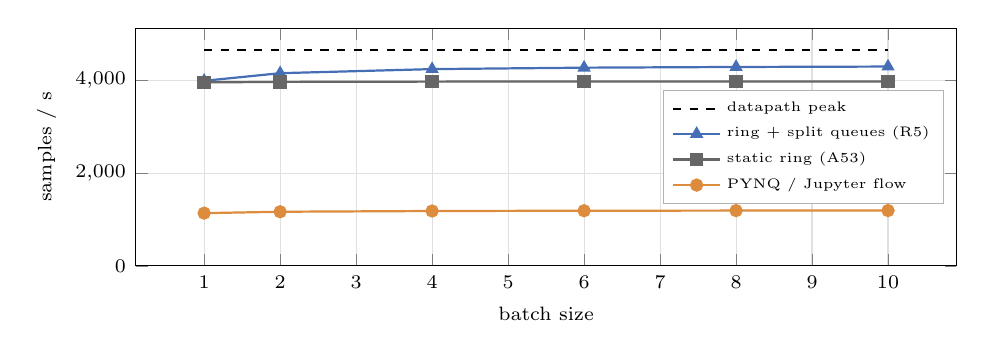
\begin{tikzpicture}
\begin{axis}[width=0.99\linewidth,height=4.6cm,
  xlabel={batch size},ylabel={samples / s},
  grid=both,grid style={black!12},ymin=0,
  tick label style={font=\scriptsize},label style={font=\scriptsize},
  legend style={font=\tiny,at={(0.985,0.5)},anchor=east,draw=black!30},
  legend cell align=left]
\addplot[dashed,black,thick] coordinates {\batchpeak};
\addlegendentry{datapath peak}
\addplot[thick,barA,mark=triangle*] coordinates {\batchtuned};
\addlegendentry{ring + split queues (R5)}
\addplot[thick,black!60,mark=square*] coordinates {\batchstatic};
\addlegendentry{static ring (A53)}
\addplot[thick,barB,mark=*] coordinates {\batchpynq};
\addlegendentry{PYNQ / Jupyter flow}
\end{axis}
\end{tikzpicture}
\caption{Throughput as a function of batch size.  Separate per-resource queues
allow the next input transfer to begin during the current computation; the
interactive flow does not recover, since every command incurs an interpreter
round trip.}
\label{fig:batch}
\end{figure}

\begin{figure}[t]
\centering
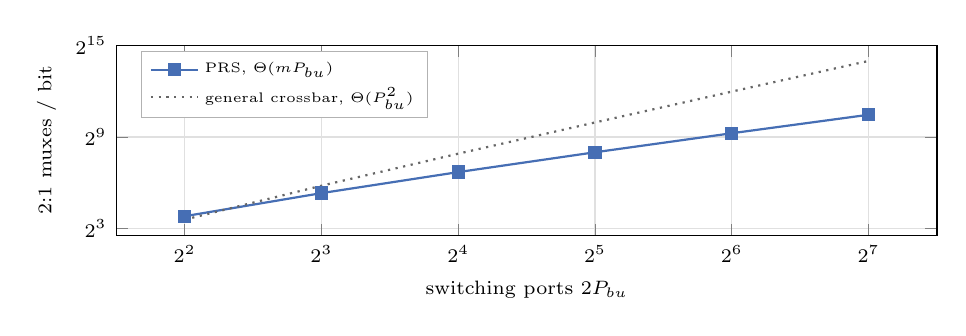
\begin{tikzpicture}
\begin{axis}[width=0.99\linewidth,height=4.0cm,
  xlabel={switching ports $2\Pbu$},ylabel={2:1 muxes / bit},
  xmode=log,log basis x=2,ymode=log,log basis y=2,
  grid=both,grid style={black!12},
  tick label style={font=\scriptsize},label style={font=\scriptsize},
  legend style={font=\tiny,at={(0.03,0.97)},anchor=north west,draw=black!30},
  legend cell align=left]
\addplot[thick,barA,mark=square*] coordinates {\prscost};
\addlegendentry{PRS, $\Theta(m\Pbu)$}
\addplot[dotted,black!60,thick] coordinates {\xbarcost};
\addlegendentry{general crossbar, $\Theta(\Pbu^2)$}
\end{axis}
\end{tikzpicture}
\caption{Switching cost of the PRS compared with a general crossbar over the
same ports.  At 128 ports the figures are \PrsMuxBig{} and \XbarMuxBig{}
multiplexers per bit respectively.  This economy is preserved under the
instruction set precisely because the schedule is kept microarchitectural.}
\label{fig:prscost}
\end{figure}

\subsection{Cost}
The sequencer adds \SeqLut{} LUTs and \SeqBram{} BRAM36 blocks to the published
system, an increase of \SeqPct\% to a total of \TotLut{} LUTs, against the
15\,k LUTs already occupied by the fixed top-level controller.  The pointwise
descriptors \op{bs.pow}, \op{bs.mag}, and \op{bs.pool} contribute
\GlueUs\,$\mu$s of computation, or \GluePct\%, which the hardwired system may
instead fuse into surrounding operations; where it does, the true overheads are
correspondingly lower than those reported here.

% ---------------------------------------------------------------------------
\section{Related Work}
Microprogrammed control originates with Wilkes~\cite{wilkes1953}, and the
present design is its accelerator-era form, in which the microinstruction is a
memory descriptor and the control store a coherent ring.  Similar arrangements
appear in the NVDLA command interface~\cite{nvdla}, the task queues of
VTA~\cite{vta}, the RoCC command stream of Gemmini~\cite{gemmini}, and the
CISC-style instructions of the TPU~\cite{tpu}.  Two features distinguish the
design presented here: the command is sized to a layer and has a closed-form
latency, and the memory schedule is deliberately excluded from the instruction
set.  Conflict-free parallel memory access for FFTs derives from
Johnson~\cite{johnson1992} and Takala et al.~\cite{takala2003} and is surveyed
by Garrido~\cite{garrido2022}.  The butterfly-linear duality that allows one
engine to serve both workloads is due to Dao et al.~\cite{dao2019butterfly} and
was first realised in hardware by FABNet~\cite{fan2022fabnet}, of which
FlexBE~\cite{flexbe}, the accelerator programmed here, is the flexible
descendant.

\section{Limitations and Future Work}
The evaluation rests on a validated model rather than on silicon.  The
sequencer's timing assumptions (Table~\ref{tab:assume}) remain to be confirmed
by board measurement, for which the natural experiment is the measurement of
three configurations on a single ZCU104---the hardwired system, the descriptor
ring, and the interactive flow---with the published RTL reused unchanged.  Two
architectural matters are acknowledged rather than resolved.  The first is
context switching in the presence of a large architectural scratchpad, which is
the customary difficulty of this class of design; for an edge appliance the
region is made process-private and non-preemptible for the duration of a
command, with save and restore through \op{bs.store} and \op{bs.load} as the
escalation path.  The second is that single-batch latency retains an irreducible
input landing time of approximately 21\,$\mu$s; this could be removed by
streaming the software-defined-radio front end directly into BSPM, an ingress
path already anticipated by the published system, which is the single most
effective improvement available.

\section{Conclusion}
A fixed-function butterfly accelerator can be made programmable by the addition
of a \SeqLut-LUT sequencer and eight opcodes, provided that the command boundary
is placed appropriately: one descriptor per layer, with shapes carried as
operands, memories and transforms exposed, and the schedule kept hidden.  On a
validated model, the resulting machine executes a complete RFML inference within
\TunedOvh\% of the hardwired datapath and sustains \TunedBatchTenPct\% of peak
throughput at a batch size of ten.  The same model further indicates that the
principal performance limitation of the deployed system lay in the
processing-system software rather than in the programmable logic.

% ---------------------------------------------------------------------------
\begin{thebibliography}{9}\footnotesize
\bibitem{flexbe} X.~Liu, R.~Wu and P.~H.~W. Leong, ``A flexible FPGA-based
butterfly engine for accelerating signal processing and machine learning,''
manuscript, The University of Sydney.
\bibitem{dao2019butterfly} T.~Dao, A.~Gu, M.~Eichhorn, A.~Rudra and C.~R\'e,
``Learning fast algorithms for linear transforms using butterfly
factorizations,'' in \emph{ICML}, 2019.
\bibitem{fan2022fabnet} H.~Fan et al., ``Adaptable butterfly accelerator for
attention-based NNs via hardware and algorithm co-design,'' in \emph{MICRO},
2022.
\bibitem{wilkes1953} M.~V. Wilkes and J.~B. Stringer, ``Micro-programming and
the design of the control circuits in an electronic digital computer,''
\emph{Proc.\ Cambridge Phil.\ Soc.}, 1953.
\bibitem{johnson1992} L.~G. Johnson, ``Conflict free memory addressing for
dedicated FFT hardware,'' \emph{IEEE TCAS-II}, 1992.
\bibitem{takala2003} J.~Takala, T.~J\"arvinen and H.~Sorokin, ``Conflict-free
parallel memory access scheme for FFT processors,'' in \emph{ISCAS}, 2003.
\bibitem{garrido2022} M.~Garrido, ``A survey on pipelined FFT hardware
architectures,'' \emph{J.\ Signal Processing Systems}, 2022.
\bibitem{tpu} N.~P. Jouppi et al., ``In-datacenter performance analysis of a
tensor processing unit,'' in \emph{ISCA}, 2017.
\bibitem{gemmini} H.~Genc et al., ``Gemmini: enabling systematic deep-learning
architecture evaluation via full-stack integration,'' in \emph{DAC}, 2021.
\bibitem{vta} T.~Moreau et al., ``A hardware--software blueprint for flexible
deep learning specialization,'' \emph{IEEE Micro}, 2019.
\bibitem{nvdla} NVIDIA, ``NVDLA deep learning accelerator,'' open-source
hardware documentation, 2017.
\end{thebibliography}

\end{document}
